\chapter{\textit{Simulação e Controle}}

Este capítulo será dedicado a relacionar o que foi falado até o momento com o projeto disponibilizado pelo MATLAB e a Parrot. Dessa forma a simulação será executada para alguns cenários de interesse e serão gerados gráficos para análise de desempenho dos controladores atuais. Assim permitindo a proposta de melhorias onde for necessário.

\section{Configuração do Modelo no MATLAB Simulink}

Para configurar o modelo no MATLAB, existe uma documentação oficial no site da mathworks*adicionar citação*, que pode ser utilizada, mas além disso uma boa proposta é seguir o trabalho de LI, David, que apresenta um forma mais simples de configuração tanto para a simulação, quanto para testar o quadricóptero físico. Nesse trabalho o objetivo é trabalhar apenas com a simulação, então para iniciar a simulação deve-se rodar o comando \textit{asbQuadcopterStart} no MATLAB, após instalar as dependências necessárias. É importante notar que a princípio as modificações que são feitas no projeto não têm nenhum intuito de melhorar a performance dos controladores ou o desempenho do modelo as configuraçôes que serão citadas a seguir só tem o papel de deixar o modelo pronto para executar as simulações com as entradas que vamos inserir e facilitar a obtenção das saídas de forma que possamos coloca-las em gráficos e realizar a análise.

\subsection{Configurando Entradas e Saídas}

Uma trajetória de voo, pode ser completamente descrita, sabendo como as coordenadas em x, y e z e a guinada do quadricóptero se comportam durante o tempo de simulação, mas como já falado na seção de controle os ângulos de rolagem e arfagem são mais importantes do que as coordenadas em x e y, quando queremos controlar o quadricóptero. Assim, é interesse desse trabalho observar o comportamento dos seis graus de liberdade que existem na simulação, as coordenadas em x, y e z, bem como rolagem, arfagem e guinada. 

\subsubsection{Configuração das entradas}

Esse modelo oferece quatro possíveis forma de entrada, Editor de Sinal, Joystick, Dados(em arquivo no formato .mat), planilha de dados(dados no formato .xlsx). Aqui como sugerido por David Li, vamos utilizar apenas editor de sinais para criar os cenários de simulação, após fazer algumas modificações necessárias para permitir a implementação correta no Simulink.

\subsubsection{Configuração de Saída}

Para as saídas, o modelo inclui estados estimados e valores de referência. No entanto, foram adicionados blocos extras, conforme descrito por Li \cite{li2022}, para incluir os valores de estado "verdadeiros" na simulação, permitindo uma comparação mais completa entre os valores estimados e simulados.

 
\section{Simulação e Resultados}

Nessa seção será apresentada a técnica utilizada para realizar as simulações, bem como os resultados obtidos na simulação.

\subsection{Simulação}

O projeto já têm dois cenários para simulação prontos dentro do bloco de edição de sinais, \textit{Hover}(Voo pairado) e \textit{Landing Search}(Voo buscando um local pré determinado para pouso). O cenário \textit{Landing Search}, não é do nosso interesse no momento pois é um cenário mais complexo, onde o drone utiliza a câmera para procurar um ponto vermelho onde deveria pousar. Como nosso interesse é estudar e entender o desempenho dos contralores, a melhor forma de obter esses resultados é com cenários mais simples como \textit{Hover}, *adicionar cenários que vão ter simulados*.

\subsubsection{Criando cenários}

Para criação ou edição de algum cenário existente, precisamos acessar o \textit{Signal Editor}, abrir o bloco \textit{Position/Attitude Reference}, e clicar no botão circulado em vermelho que abrirá o editor de sinais.


\begin{figure}[H]
	\centering
	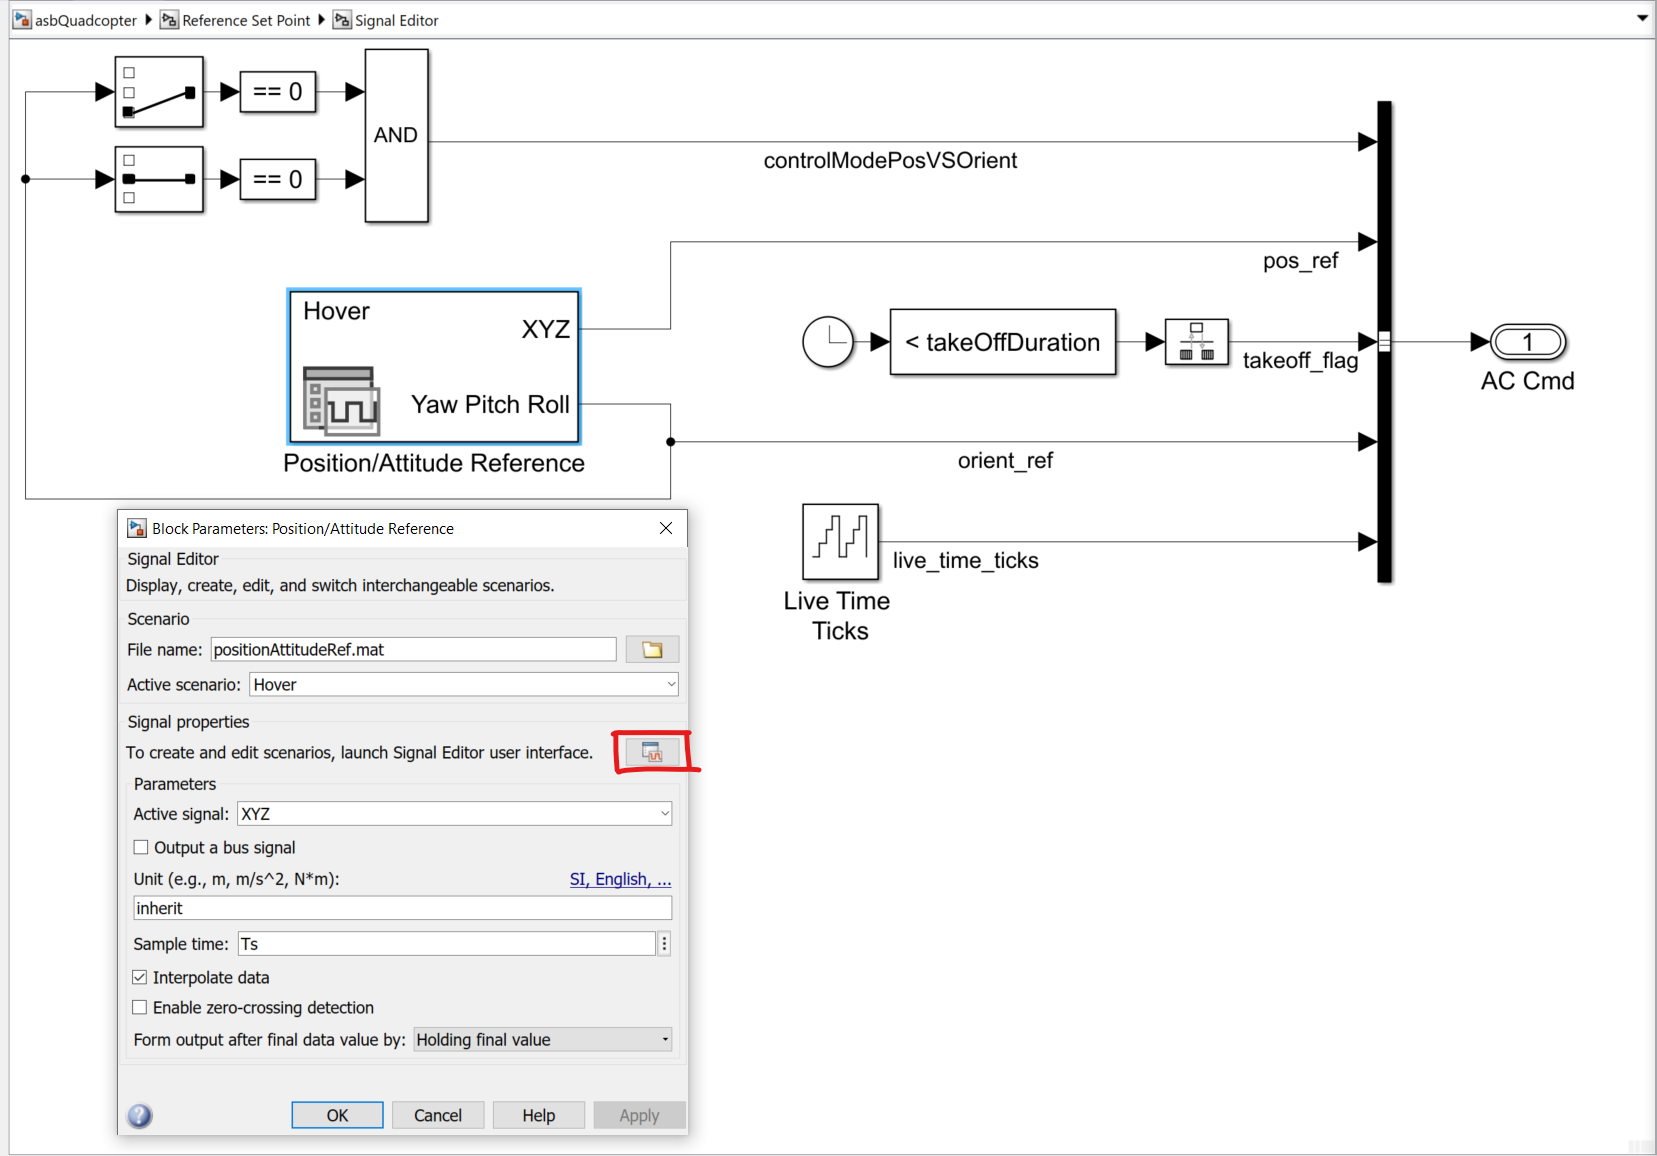
\includegraphics[width=1\textwidth]{signal-editor-open.png}
	\caption{Como abrir o Editor de Sinais}
	\centering
	\label{sinal-editor-open}
\end{figure}

No editor de sinais, podemos inserir nossos dados de entrada, para os nossos seis graus de liberdade, e em qual momento da simulação o sinal será enviado.


\begin{figure}[H]
	\centering
	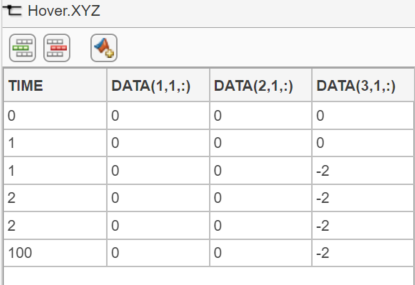
\includegraphics[width=1\textwidth]{signal-editor-xyz-hover.png}
	\caption{Modificando cenários de Simulação X Y Z}
	\centering
	\label{sinal-editor-xyz-hover}
\end{figure}

\begin{figure}[H]
	\centering
	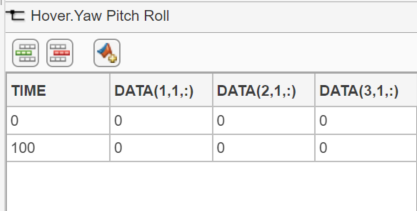
\includegraphics[width=1\textwidth]{signal-editor-pry-hover.png}
	\caption{Modificando cenários de Simulação Guinada, Arfagem e Rolagem}
	\centering
	\label{signal-editor-pry-hover}
\end{figure}


Para executar os cenários de forma programática e pegar os resultados, utilizaremos um código retirado também da nossa principal referência nesse capítulo.

\begin{lstlisting}[language=Matlab, caption={Configuração de Cenários no MATLAB Simulink}]
	scenarios = {'TesteXY3'; 'LandingSearch'};
	TFinals = [25;30];
	
	in = Simulink.SimulationInput.empty(size(scenarios, 1), 0);
	for i = 1 : size(scenarios, 1)
		in(i) = Simulink.SimulationInput('asbQuadcopter');
		in(i) = in(i).setBlockParameter(['flightControlSystem/Flight Control System/' ...
			'landing logic/Position//Attitude Reference'], ...
			'ActiveScenario', scenarios{i});
		in(i) = in(i).setVariable('TFinal', TFinals(i), 'Workspace', 'asbQuadcopter');
	end
	
	out = sim(in(1)); % simulate with the "Hover" scenario for 10 seconds
\end{lstlisting}

No código acima, as linhas 1 e 2 definem o cenário que pretendemos simular(previamente criado dentro do editor de sinais), e o tempo de simulação, respectivamente. O laço de repetição da linha 5 a 11, coloca o cenário no bloco Position/Attitude Reference que está dentro de \textit{Landing logic}, que foi inserido após as modificações que seguimos na seção \textit{configuraçôes de entrada}. A linha 13, executa a simulação com o cenário escolhido e salva os resultados na variável \textit{out}.

A variável \textit{out}, contém todas as informações que são do nosso interesse, no seguinte formato:

\begin{lstlisting}[language=Matlab, caption={Exemplo de extração de dados simulados}, numbers=left, backgroundcolor=\color{lightgray}]
	t = out.posref.time;
	xyzrpy = out.xyzrpy;
	estim = out.estim.signals.values;
	posref = out.posref.signals.values;
	motor = out.motor.signals.values;
	sensor = out.sensor.signals.values;
\end{lstlisting}

Com isso, agora podemos executar os cenários com facilidade e colocar os resultados de forma gráfica, para observamos o comportamento dos controladores.

\subsection{Resultados}

Nesta seção, será realizada a análise dos gráficos gerados a partir das simulações realizadas no MATLAB Simulink. O objetivo principal é avaliar o desempenho dos controladores do quadricóptero em diferentes cenários, com foco no comportamento das variáveis de interesse, como a posição \(x\), \(y\), \(z\) e os ângulos de rolagem, arfagem e guinada.

Para interpretar os gráficos de desempenho, serão consideradas as seguintes métricas:
\begin{itemize}
    \item \textbf{Tempo de estabilização}: Tempo necessário para que o sistema se estabilize após uma mudança de referência ou perturbação.
    \item \textbf{Overshoot (ultrapassagem)}: A porcentagem que a resposta do sistema excede o valor de referência antes de se estabilizar.
    \item \textbf{Erro em regime permanente}: A diferença entre o valor final da variável controlada e o valor de referência após o sistema estabilizar.
    \item \textbf{Tempo de subida}: O tempo que o sistema leva para sair de 10\% a 90\% do valor final após uma mudança de referência.
\end{itemize}

Essas métricas permitirão avaliar a eficácia dos controladores em manter o quadricóptero estável e responsivo, principalmente no cenário de voo pairado (\textit{Hover}), onde a precisão de posição e estabilidade são cruciais.

Os gráficos apresentam o comportamento das coordenadas do quadricóptero ao longo do tempo nos cenários de interesse montados. Ele compara três curvas: \textbf{Posição verdadeiro} (linha azul), que representa a altura real do quadricóptero; \textbf{Posição estimado} (linha laranja), que é a estimativa feita pelo sistema; e \textbf{Posição referência} (linha amarela), que é o valor de referência.

Nas curvas de atitude, é necessário elucidar melhor os termos os termos utilizados. Assim, aqui é preciso lembrar que para o quadricóptero realizar movimentos horinzontais, é necessário que aconteça uma arfagem ou rolagem, e no controlador de voo, temos um subsistema que converte os valore de de referência de x e y, em comandos de rolagem e arfagem. Nos gráficos, a resultande desses valores são chamados de  \textbf{comando de arfagem} e \textbf{comando de rolagem}.

\subsubsection{Voo Pairado (Hover)}

Neste cenário de voo pairado, o objetivo é que o drone suba até uma altura determinada e permaneça nessa altura até o fim da simulação. Além de analisar o desempenho do controlador de altitude, é interessante observar o comportamento dos controladores de posição nos eixos \(X\) e \(Y\), além dos controladores de arfagem, guinada e rolagem.

Parâmetros da simulação: \\

- Tempo total: 25 segundos;\\
- Altura desejada: 2 metros; \\
- Posição em \(X\) e \(Y\): 0.

1) Coordenada Z

\begin{figure}[H]
	\centering
	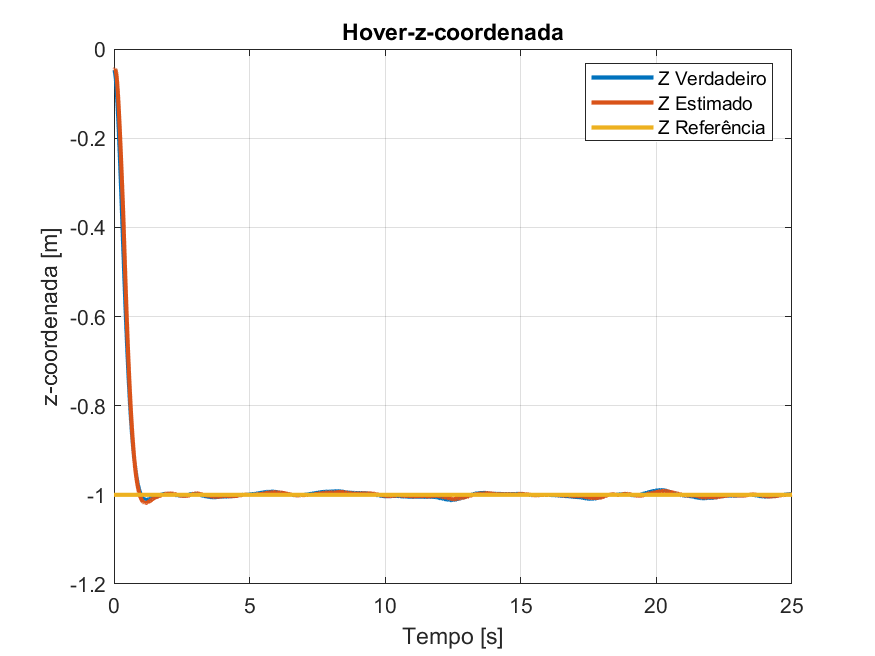
\includegraphics[width=1\textwidth]{Hover-z-coordenada.png}
	\caption{Coordenada Z para o Cenário de Voo Pairado}
	\label{fig:hover-z-coordenada}
\end{figure}

Analisando o gráfico, podemos observar que o tempo de estabilização é rápido, por volta dos 3 segundos, após o qual o sistema atinge a estabilidade próximo ao valor de referência. Um pequeno overshoot é visível no início, mas é bem controlado, e o erro em regime permanente é mínimo, indicando um bom desempenho do controlador para manter a altitude.

2) Coordenadas X e Y

Abaixo estão os gráficos das coordenadas \(X\) e \(Y\) do quadricóptero ao longo do tempo:

\begin{figure}[htbp]
    \centering
    \subfloat[Coordenada X para o Cenário de Voo Pairado]{
        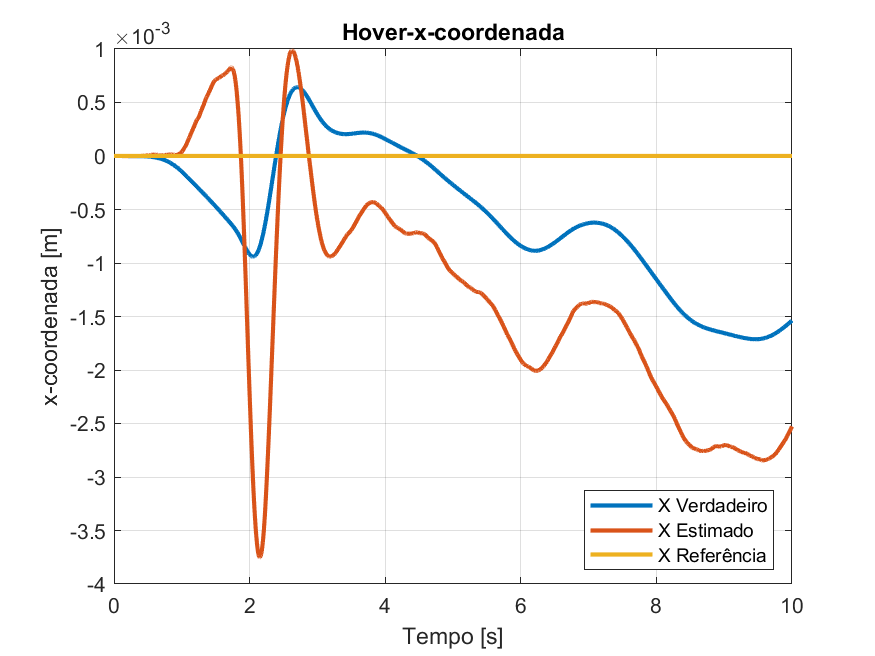
\includegraphics[width=0.45\textwidth]{Hover-x-coordenada.png}
        \label{fig:hover-x-coordenada}
    }
    \hfill
    \subfloat[Coordenada Y para o Cenário de Voo Pairado]{
        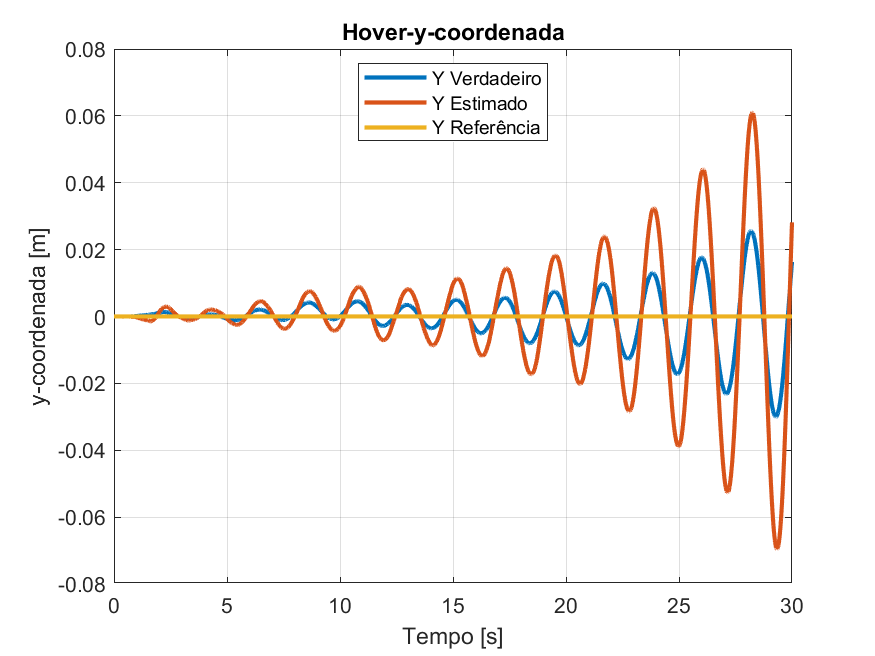
\includegraphics[width=0.45\textwidth]{Hover-y-coordenada.png}
        \label{fig:hover-y-coordenada}
    }
    \caption{Coordenadas X e Y para o Cenário de Voo Pairado}
    \label{fig:hover-x-y-coordenadas}
\end{figure}

No dois gráficos, podemos observar oscilações crescentes em torno do valor de referência com o tempo. No gráfico do eixo \(Y\), vemos que o valor verdadeiro aumenta ao longo do tempo proporcionalmente com os valores estimados, na curva de \(X\), apesar das altas oscilações dos valores estimados, o valor verdadeiro consegue se manter próximo ao valor de referência.

%Para ambos os eixos, uma possível solução é ajustar os ganhos \(K_p\) e \(K_d\) para suavizar a resposta e aumentar o amortecimento, além de adicionar um ganho integral \(K_i\) para reduzir o erro em regime permanente.

3) Ângulos de Rolagem, Arfagem e Guinada

A seguir estão os gráficos para os ângulos de rotação do quadricóptero: rolamento (roll), arfagem (pitch) e guinada (yaw).

\begin{figure}[htbp]
    \centering
    \subfloat[Arfagem para o Cenário de Voo Pairado]{
        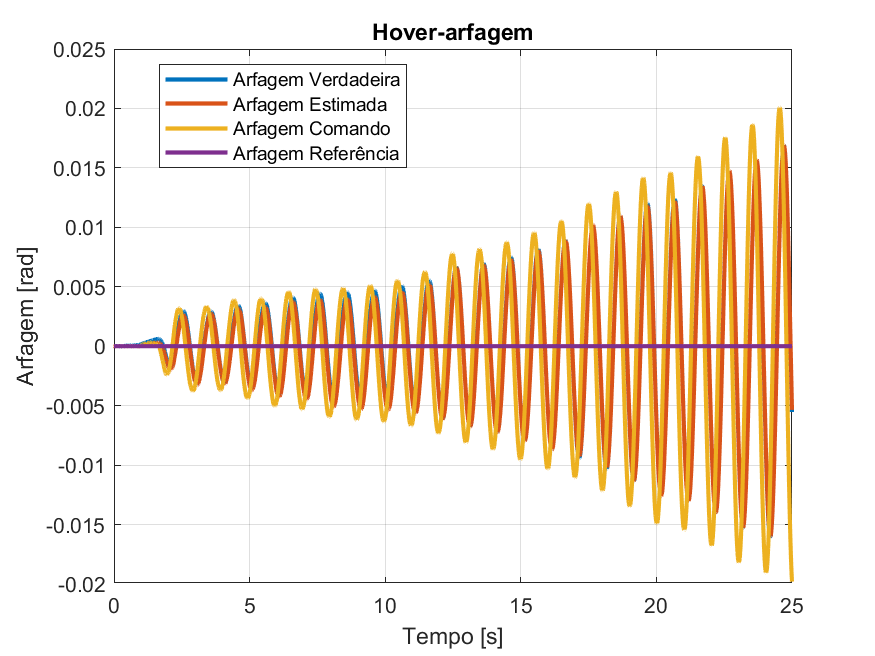
\includegraphics[width=0.45\textwidth]{Hover-arfagem.png}
        \label{fig:hover-arfagem}
    }
    \hfill
    \subfloat[Guinada para o Cenário de Voo Pairado]{
        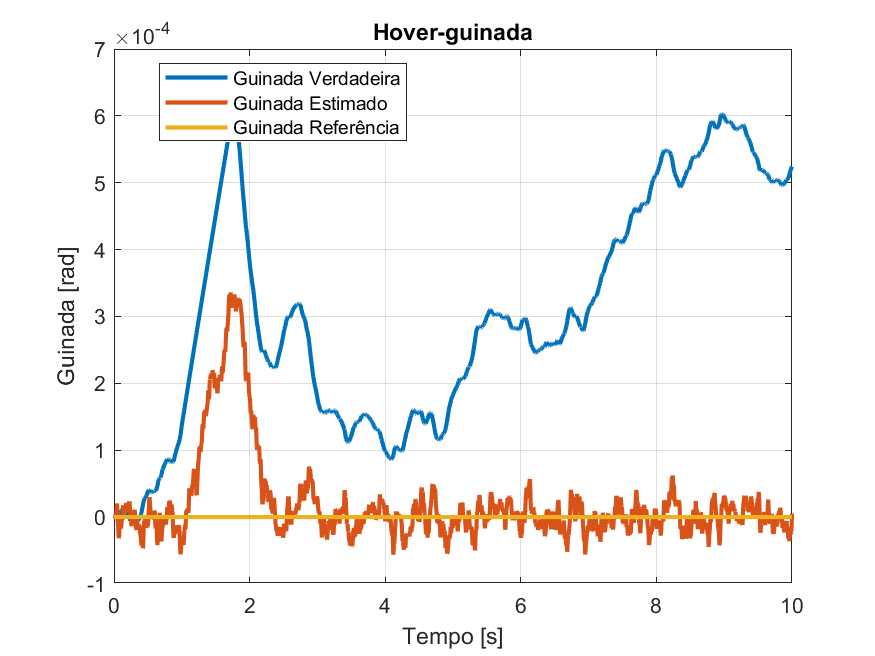
\includegraphics[width=0.45\textwidth]{Hover-guinada.png}
        \label{fig:hover-guinada}
    }
    \caption{Arfagem e Guinada para o Cenário de Voo Pairado}
    \label{fig:hover-arfagem-guinada}
\end{figure}

\begin{figure}[H]
	\centering
	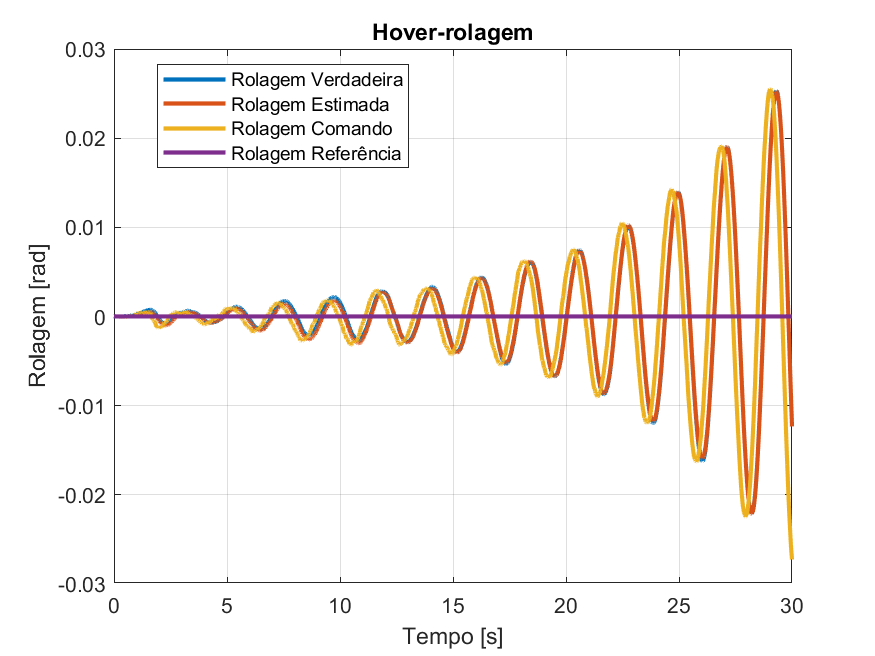
\includegraphics[width=0.5\textwidth]{Hover-rolagem.png}
	\caption{Rolagem para o Cenário de Voo Pairado}
	\label{fig:hover-rolagem}
\end{figure}

Nos gráficos, vemos que os ângulos de arfagem e rolamento apresentam oscilações crescentes ao longo do tempo, o que inclusive concorda com o comportamento que observamos nos eixos  \(X\) e  \(Y\) ,enquanto o ângulo de guinada permanece relativamente estável. Essas oscilações indicam uma possível falta de amortecimento no controlador, especialmente nos eixos de arfagem e rolamento.

Sendo assim, uma boa estratégia para iniciarmos nossas melhorias seria ajustar os parâmetros dos controladores de arfagem e rolagem, bem como os contralores da posição \(X\) e \(Y\).



%Para melhorar o desempenho, recomenda-se ajustar os parâmetros do controlador para reduzir as oscilações nesses eixos, aplicando amortecimento adicional e revisando os ganhos de controle. Isso deve resultar em um sistema mais estável e menos propenso a oscilações crescentes.

%Conclusão Geral para o Cenário de Voo Pairado

%No cenário de voo pairado, o controlador de altitude apresenta um bom desempenho, mas os controladores de posição e atitude nos eixos \(X\) e \(Y\), assim como os controladores de rotação (roll e pitch), mostram sinais de instabilidade. Ajustes nos parâmetros de controle são recomendados para melhorar a resposta geral e a estabilidade do sistema, especialmente em situações que exigem controle preciso de posição e orientação.




%---------------------------------------------------------------------
% INDICE REMISSIVO
%---------------------------------------------------------------------
\phantompart
\printindex
%---------------------------------------------------------------------

%\subsubsection{Mudança de Altitude (Altitude Change)}

Neste cenário de mudança de altitude, o objetivo é que o drone ajuste sua altura em resposta a uma nova referência de altitude, mantendo-se estável nas posições \(X\) e \(Y\) durante essa mudança. Além de analisar o desempenho do controlador de altitude, também é importante observar como os controladores de posição e atitude reagem a essa transição.

Parâmetros da simulação: \\

- Tempo total: 25 segundos;\\
- Altura inicial: 2 metros; \\
- Altura desejada: 1 metros; \\
- Posição em \(X\) e \(Y\): 0, 0. \\
- t mudança de altitude: 2s



1) Coordenada Z

O gráfico abaixo mostra o comportamento da coordenada \(Z\) ao longo do tempo.

\begin{figure}[H]
	\centering
	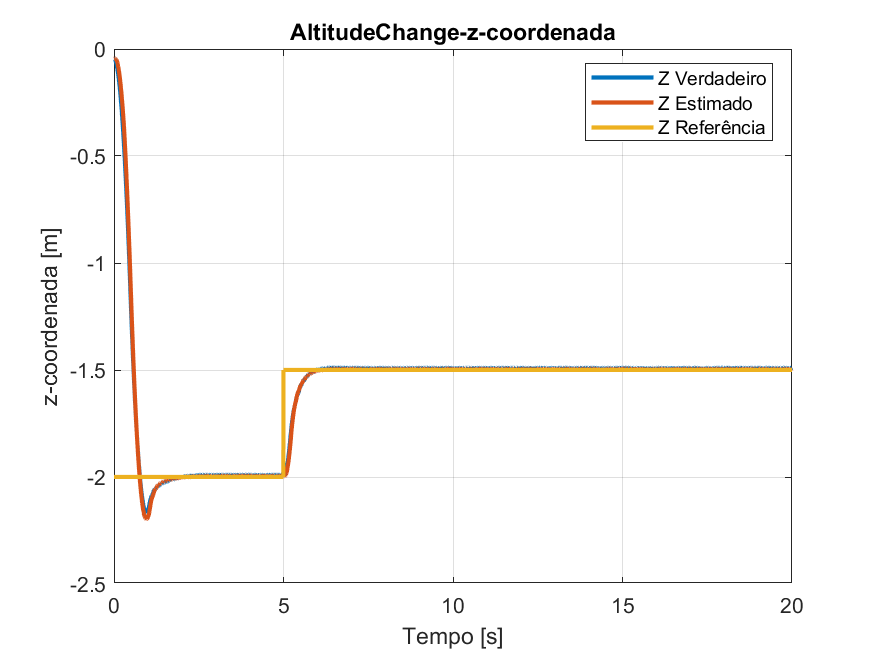
\includegraphics[width=1\textwidth]{AltitudeChange-z-coordenada.png}
	\caption{Coordenada Z para o Cenário de Mudança de Altitude}
	\label{fig:altitudechange-z-coordenada}
\end{figure}

Observamos que o sistema atinge a nova referência de altitude rapidamente, com um pequeno overshoot após a mudança de altitude. A estabilização ocorre após aproximadamente 5 segundos. Esse comportamento indica um bom desempenho do controlador de altitude para alcançar o valor de referência com um erro em regime permanente praticamente nulo.

2) Coordenadas X e Y

Os gráficos a seguir mostram o comportamento das coordenadas \(X\) e \(Y\) ao longo do tempo, permitindo uma análise do controle de posição durante a mudança de altitude.

\begin{figure}[htbp]
    \centering
    \subfloat[Coordenada X para o Cenário de Mudança de Altitude]{
        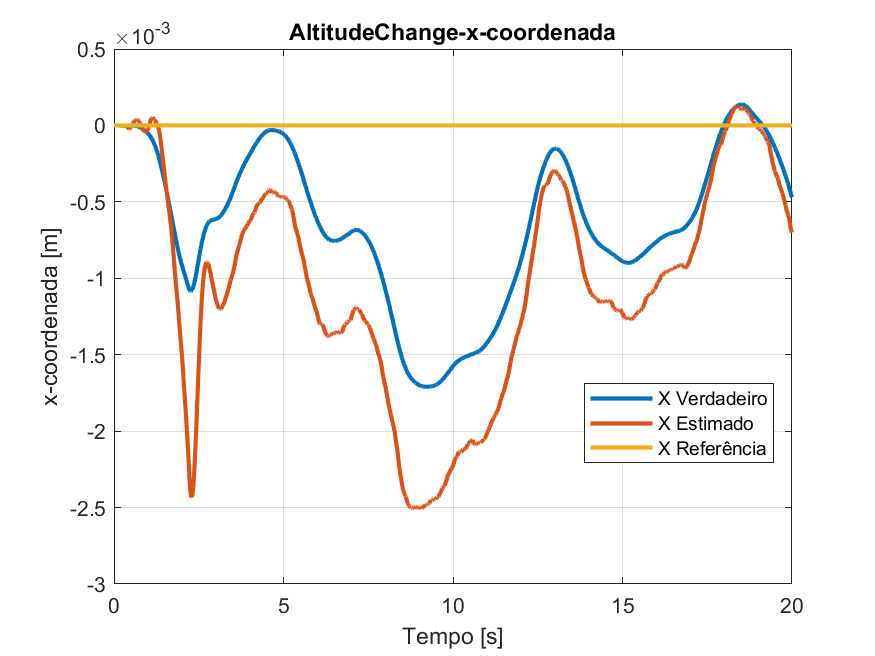
\includegraphics[width=0.45\textwidth]{AltitudeChange-x-coordenada.png}
        \label{fig:altitudechange-x-coordenada}
    }
    \hfill
    \subfloat[Coordenada Y para o Cenário de Mudança de Altitude]{
        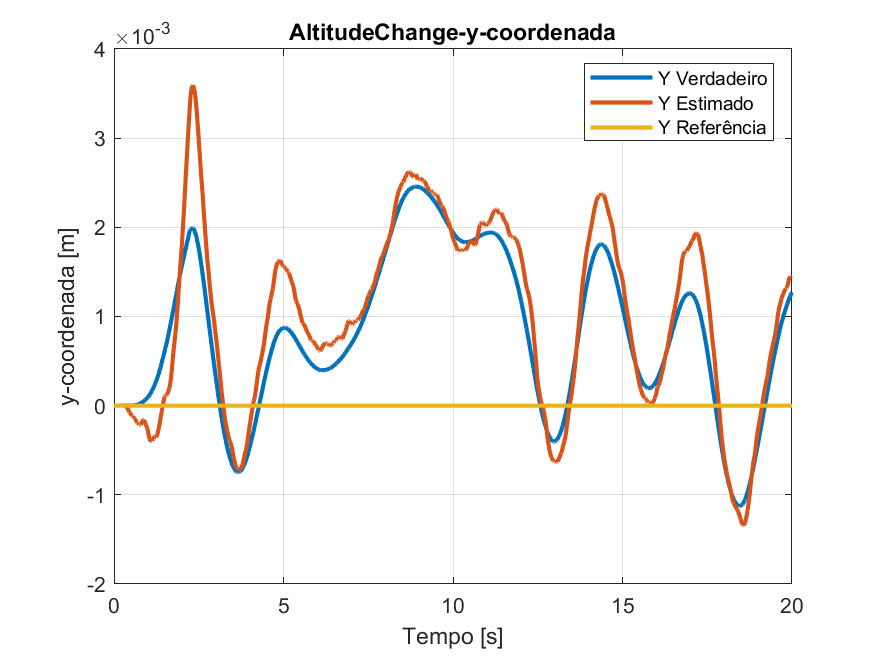
\includegraphics[width=0.45\textwidth]{AltitudeChange-y-coordenada.png}
        \label{fig:altitudechange-y-coordenada}
    }
    \caption{Coordenadas X e Y para o Cenário de Mudança de Altitude}
    \label{fig:altitudechange-x-y-coordenadas}
\end{figure}

Nos gráficos das coordenadas \(X\) e \(Y\), observamos que, durante a mudança de altitude, as posições \(X\) e \(Y\) nâo exibem oscilações significativas, na ordem dos milímetros, em torno da posição de referência. A curva de estimativa de posição \(Y\) (linha laranja) tem uma amplitude de oscilação baixa em comparação com a curva verdadeira e podemos ver que a amplitiude diminui com o tempo. No gráfico de \(X\), o comportamento é semelhante, com oscilações que diminuem progressivamente em direção a estabilidade.

Essas oscilações mostran que o sistema de controle de posição consegue manter a estabilidade durante a transição de altitude. Sendo interessante notar que o sistema de comporta melhor após a mudança de altitude do que num voo pairado, sendo assim, ao realizar nossos ajustes no sistema para melhorar o desempenho em voo pairado, devemos tomar cuidado para não prejudicar o sistema em um cenário de mudança de altitude..

3) Ângulos de Rolagem, Arfagem e Guinada

Os gráficos a seguir mostram os ângulos de rolamento (roll), arfagem (pitch) e guinada (yaw) do quadricóptero durante a mudança de altitude.

\begin{figure}[htbp]
    \centering
    \subfloat[Arfagem para o Cenário de Mudança de Altitude]{
        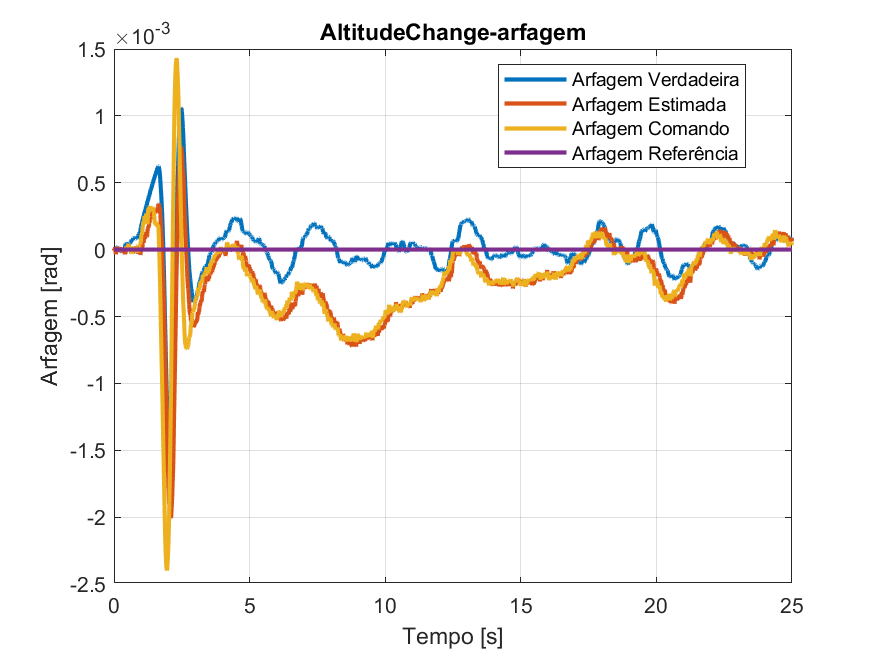
\includegraphics[width=0.45\textwidth]{AltitudeChange-arfagem.png}
        \label{fig:altitudechange-arfagem}
    }
    \hfill
    \subfloat[Guinada para o Cenário de Mudança de Altitude]{
        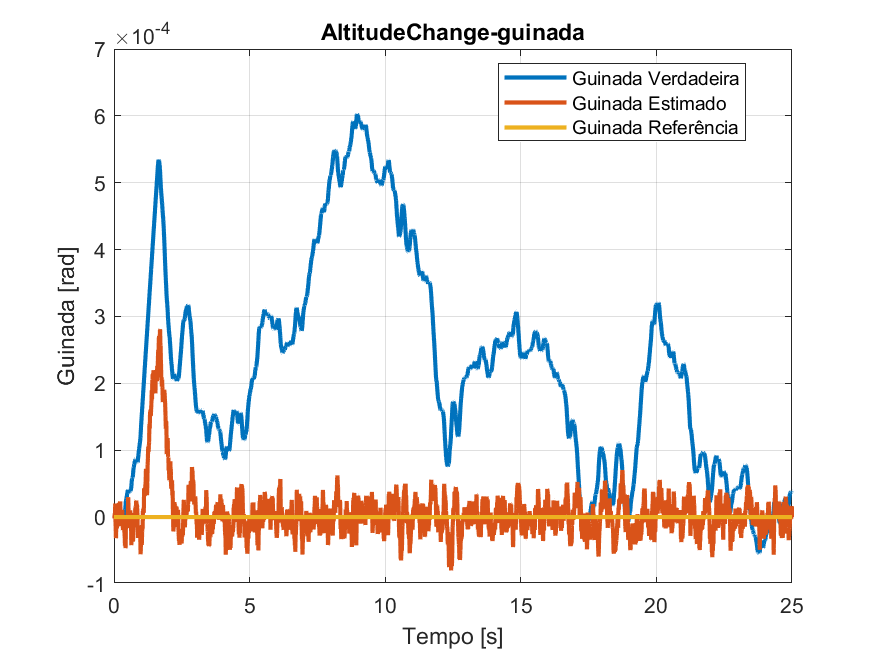
\includegraphics[width=0.45\textwidth]{AltitudeChange-guinada.png}
        \label{fig:altitudechange-guinada}
    }
    \caption{Arfagem e Guinada para o Cenário de Mudança de Altitude}
    \label{fig:altitudechange-arfagem-guinada}
\end{figure}

\begin{figure}[H]
	\centering
	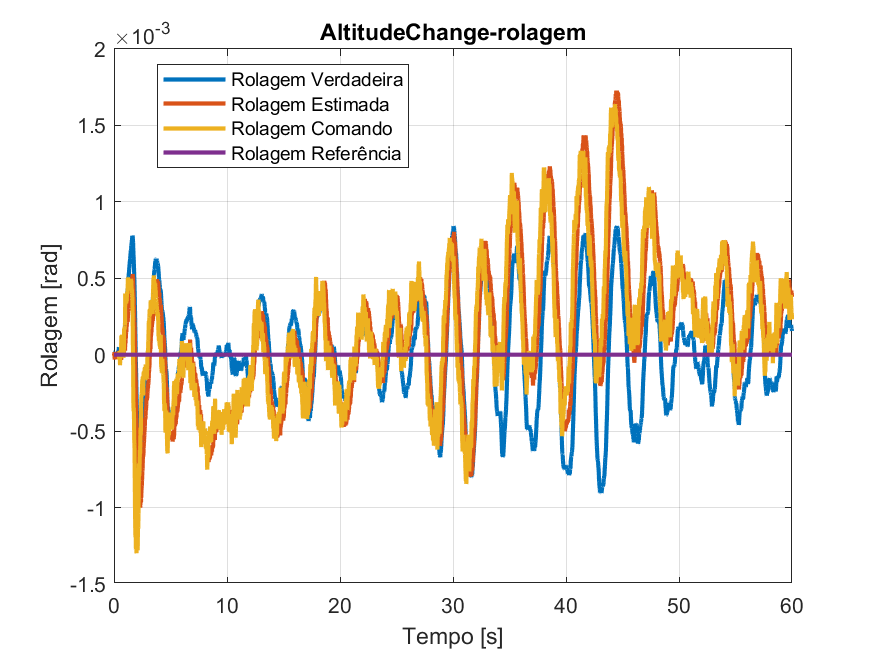
\includegraphics[width=0.5\textwidth]{AltitudeChange-rolagem.png}
	\caption{Rolagem para o Cenário de Mudança de Altitude}
	\label{fig:altitudechange-rolagem}
\end{figure}

Durante a transição de altitude, os ângulos de arfagem e rolamento apresentam oscilações notáveis, mas de baixa amplitude. No gráfico de arfagem e de rolagem, observa-se um comportamento oscilatório acentuado no momento da mudança de altitude,mas que com o tempo tende a estabilidade em torno do valor de referência, o que indica que o controlador precisa ser ajustado para responder de forma mais suave. O gráfico de guinada mostra variações menores, o que sugere um controle mais estável para esse eixo.

%A amplitude das oscilações em rolamento e arfagem indica que o sistema de controle está mal ajustado para esses eixos durante a transição de altitude. Ajustes nos parâmetros de controle, como o ganho derivativo \(K_d\), poderiam ajudar a reduzir essas oscilações e melhorar a resposta do sistema.

%### Conclusão Geral para o Cenário de Mudança de Altitude

%No cenário de mudança de altitude, o controlador de altitude funciona bem, atingindo o novo valor de referência de forma rápida e com mínimo erro em regime permanente. No entanto, os controladores de posição nos eixos \(X\) e \(Y\) e os controladores de atitude nos eixos de rolamento e arfagem exibem sinais de instabilidade, com oscilações crescentes ao longo do tempo. Para melhorar o desempenho, recomenda-se um ajuste nos ganhos do controlador, especialmente nos eixos \(X\) e \(Y\), bem como nos controladores de atitude, para reduzir as oscilações e melhorar a estabilidade geral do sistema.


%---------------------------------------------------------------------
% INDICE REMISSIVO
%---------------------------------------------------------------------
\phantompart
\printindex
%---------------------------------------------------------------------

%\subsubsection{Altidude Constante seguido de Arfagem}

Neste cenário, o objetivo é que o quadricóptero mantenha uma atitude fixa em arfagem (\textit{pitch}) enquanto estabiliza a altitude e as posições \(X\) e \(Y\). A análise considera a resposta dos controladores para cada uma dessas variáveis, observando-se as trajetórias real, estimada e de referência.

Parâmetros da simulação: \\

- Tempo total: 30 segundos;\\
- Altura desejada: 2 metros; \\
- Arfagem de 0.1 rad(5,73 graus) em t =5s

1) Arfagem

O gráfico a seguir mostra o comportamento do ângulo de arfagem ao longo do tempo.

\begin{figure}[H]
	\centering
	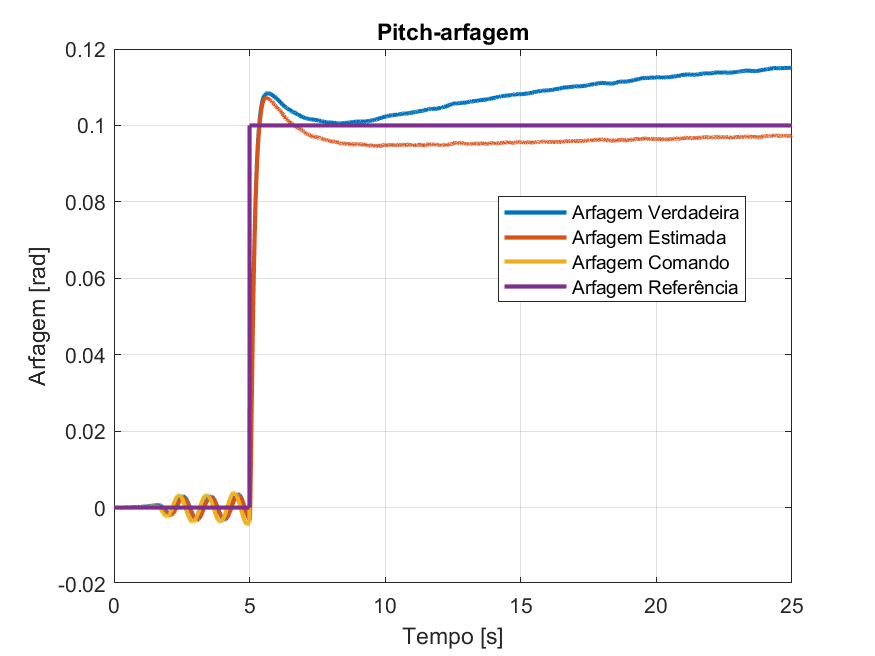
\includegraphics[width=0.8\textwidth]{Pitch-arfagem.png}
	\caption{Arfagem para o Cenário de Pitch}
	\label{fig:pitch-arfagem}
\end{figure}

Neste gráfico, observamos que o ângulo de arfagem responde rapidamente ao comando de referência, alcançando um valor de aproximadamente \(0.1\) radianos. Contudo, notamos uma pequena diferença entre a curva verdadeira (linha azul) e a estimada (linha laranja) após a arfagem. Essa diferença indica uma leve defasagem entre o valor verdadeiro e o valor estimado. A curva de referência (linha roxa) permanece constante, indicando o ângulo alvo desejado para este cenário.

2) Coordenada X

A seguir, temos o gráfico da posição \(X\) do quadricóptero ao longo do tempo.

\begin{figure}[H]
	\centering
	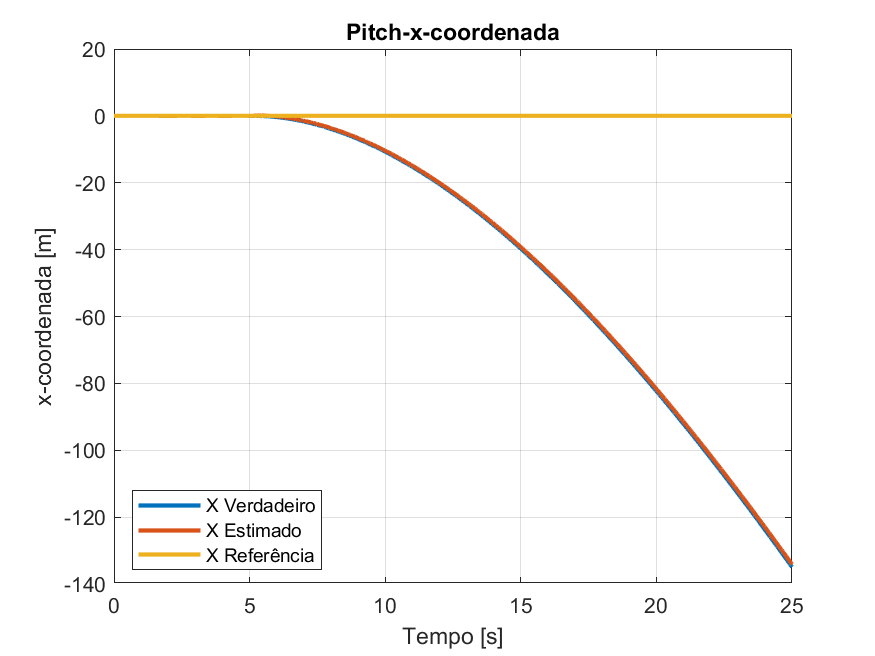
\includegraphics[width=0.8\textwidth]{Pitch-x-coordenada.png}
	\caption{Coordenada X para o Cenário de Pitch}
	\label{fig:pitch-x-coordenada}
\end{figure}

A posição \(X\) mostra um comportamento de translação contínua ao longo do tempo, conforme esperado para um cenário de arfagem constante, onde o quadricóptero se desloca em direção ao eixo \(X\). As curvas verdadeira e estimada (linhas azul e laranja) coincidem bem, indicando uma boa precisão na estimativa de posição.

3) Coordenada Z

Por fim, analisamos o comportamento da coordenada \(Z\) ao longo do tempo.

\begin{figure}[H]
	\centering
	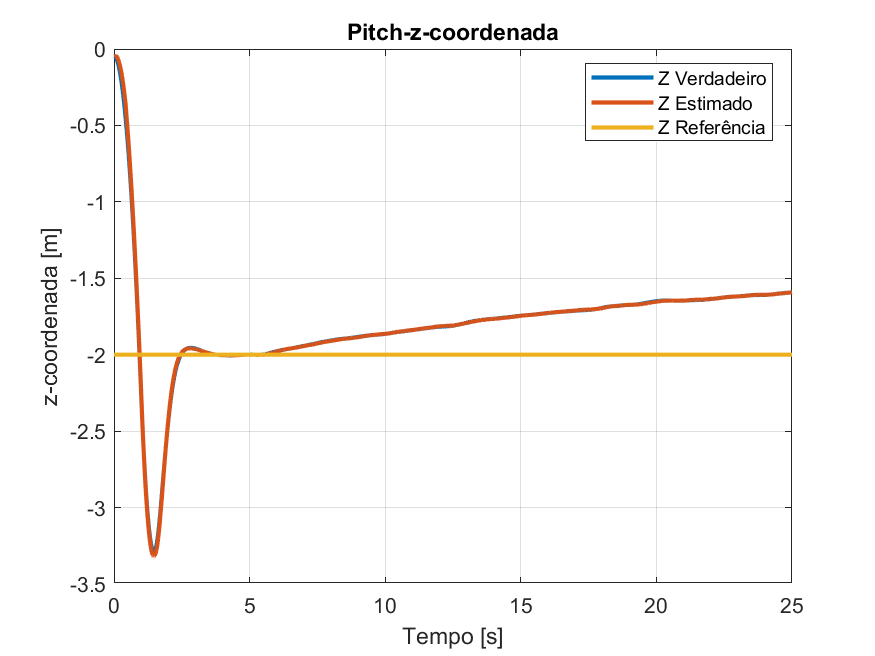
\includegraphics[width=0.8\textwidth]{Pitch-z-coordenada.png}
	\caption{Coordenada Z para o Cenário de Pitch}
	\label{fig:pitch-z-coordenada}
\end{figure}

Neste gráfico, a altitude mostra uma leve tendência de aumento com o passar do tempo, ainda que a referência de altura permaneça constante. A diferença entre as curvas verdadeira e estimada mostra que o sistema de controle está encontrando dificuldade para manter a altitude estável quando a inclinação de pitch é aplicada.

%### Conclusão Geral para o Cenário de Pitch

%O cenário de pitch revela um bom desempenho na estimativa de posição \(X\) e \(Y\), com ambas as curvas de posição verdadeira e estimada acompanhando bem a referência ao longo do tempo. No entanto, o controle de altitude apresenta uma leve instabilidade, o que pode exigir ajustes nos parâmetros do controlador para evitar desvios indesejados na coordenada \(Z\). Além disso, a leve diferença entre as curvas de arfagem verdadeira e estimada sugere que ajustes no controlador de pitch poderiam melhorar ainda mais a precisão da resposta do sistema.


%---------------------------------------------------------------------
% INDICE REMISSIVO
%---------------------------------------------------------------------
\phantompart
\printindex
%---------------------------------------------------------------------

%\subsubsection{Altidude Constante seguido de Rolagem}

Neste cenário, o objetivo é que o quadricóptero mantenha uma atitude fixa em arfagem (\textit{pitch}) enquanto estabiliza a altitude e as posições \(X\) e \(Y\). A análise considera a resposta dos controladores para cada uma dessas variáveis, observando-se as trajetórias real, estimada e de referência.

Parâmetros da simulação: \\

- Tempo total: 30 segundos;\\
- Altura desejada: 2 metros; \\
- Rolagem de 0.1 rad(5,73 graus) em t =5s

1) Rolagem

O gráfico a seguir mostra o comportamento do ângulo de arfagem ao longo do tempo.

\begin{figure}[H]
	\centering
	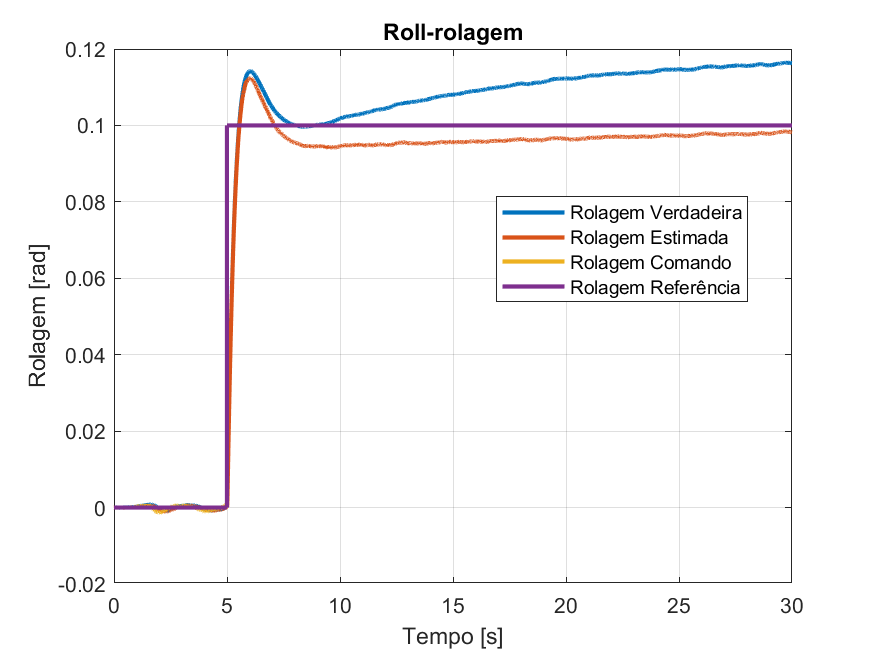
\includegraphics[width=0.8\textwidth]{Roll-rolagem.png}
	\caption{Rolagem para o Cenário de rolagem}
	\label{fig:roll-arfagem}
\end{figure}

Neste gráfico, observamos que o ângulo de arfagem responde rapidamente ao comando de referência, alcançando um valor de aproximadamente \(0.1\) radianos. Contudo, notamos uma pequena diferença entre a curva verdadeira (linha azul) e a estimada (linha laranja) após a rolagem. Essa diferença indica uma leve defasagem entre o valor verdadeiro e o valor estimado. A curva de referência (linha roxa) permanece constante, indicando o ângulo alvo desejado para este cenário.

2) Coordenada Y

A seguir, temos o gráfico da posição \(Y\) do quadricóptero ao longo do tempo.

\begin{figure}[H]
	\centering
	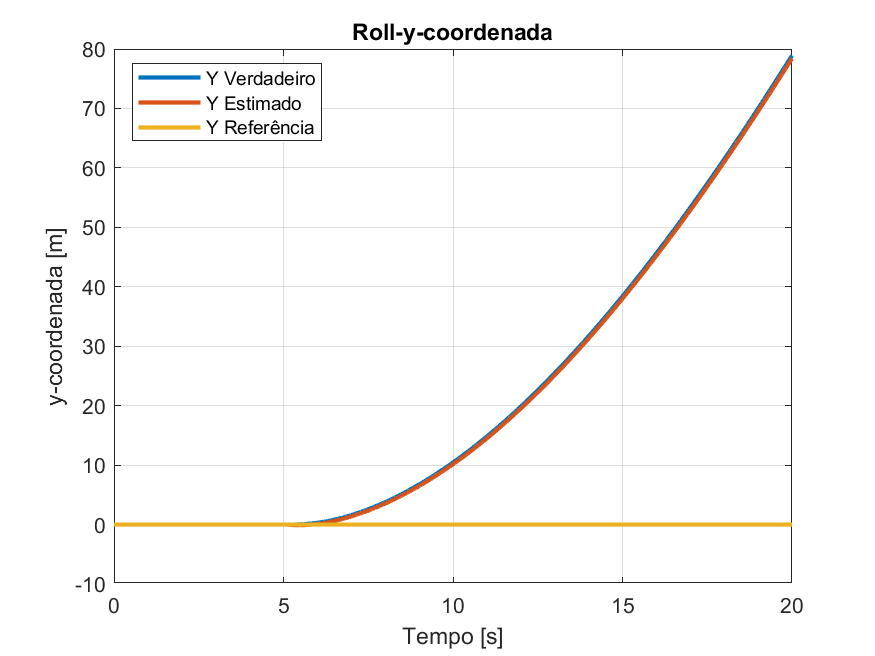
\includegraphics[width=0.8\textwidth]{Roll-y-coordenada.png}
	\caption{Coordenada Y para o Cenário de rolagem}
	\label{fig:roll-x-coordenada}
\end{figure}

A posição \(X\) mostra um comportamento de translação contínua ao longo do tempo, conforme esperado para um cenário de arfagem constante, onde o quadricóptero se desloca em direção ao eixo \(X\). As curvas verdadeira e estimada (linhas azul e laranja) coincidem bem, indicando uma boa precisão na estimativa de posição.

3) Coordenada Z

Por fim, analisamos o comportamento da coordenada \(Z\) ao longo do tempo.

\begin{figure}[H]
	\centering
	\includegraphics[width=0.8\textwidth]{roll-z-coordenada.png}
	\caption{Coordenada Z para o Cenário de Rolagem}
	\label{fig:roll-z-coordenada}
\end{figure}

Neste gráfico, a altitude mostra uma leve tendência de aumento com o passar do tempo, ainda que a referência de altura permaneça constante. A diferença entre as curvas verdadeira e estimada mostra que o sistema de controle está encontrando dificuldade para manter a altitude estável quando a inclinação de pitch é aplicada.

%### Conclusão Geral para o Cenário de Pitch

%O cenário de pitch revela um bom desempenho na estimativa de posição \(X\) e \(Y\), com ambas as curvas de posição verdadeira e estimada acompanhando bem a referência ao longo do tempo. No entanto, o controle de altitude apresenta uma leve instabilidade, o que pode exigir ajustes nos parâmetros do controlador para evitar desvios indesejados na coordenada \(Z\). Além disso, a leve diferença entre as curvas de arfagem verdadeira e estimada sugere que ajustes no controlador de pitch poderiam melhorar ainda mais a precisão da resposta do sistema.


%---------------------------------------------------------------------
% INDICE REMISSIVO
%---------------------------------------------------------------------
\phantompart
\printindex
%---------------------------------------------------------------------


%---------------------------------------------------------------------
% INDICE REMISSIVO
%---------------------------------------------------------------------
\phantompart
\printindex
%---------------------------------------------------------------------
